% Diagram of Android activity life cycle
% Author: Pavel Seda 
\documentclass[border=10pt]{standalone}
%%%<
\usepackage{verbatim}
\newcommand{\tss}{\textsuperscript}
\newcommand{\tsbs}{\textsubscript}
%%%>
\begin{comment}
:Title: Diagram of Android activity life cycle
:Tags: Diagrams;Flowcharts;Charts;Styles;Computer science
:Author: Pavel Seda
:Slug: android

A flow diagram of an Android activity life cycle.
It uses basic nodes and arrows and defines node styles.
\end{comment}
\usepackage{tikz}
\usetikzlibrary{arrows.meta}
\tikzset{%
  >={Latex[width=2mm,length=2mm]},
  % Specifications for style of nodes:
            base/.style = {rectangle, rounded corners, draw=black,
                           minimum width=4cm, minimum height=1cm,
                           text centered, font=\sffamily},
  activityStarts/.style = {base, fill=blue!30},
       startstop/.style = {base, fill=red!30},
    activityRuns/.style = {base, fill=green!30},
         process/.style = {base, minimum width=2.5cm, fill=orange!15,
                           font=\ttfamily},
}
\begin{document}    
% Drawing part, node distance is 1.5 cm and every node
% is prefilled with white background
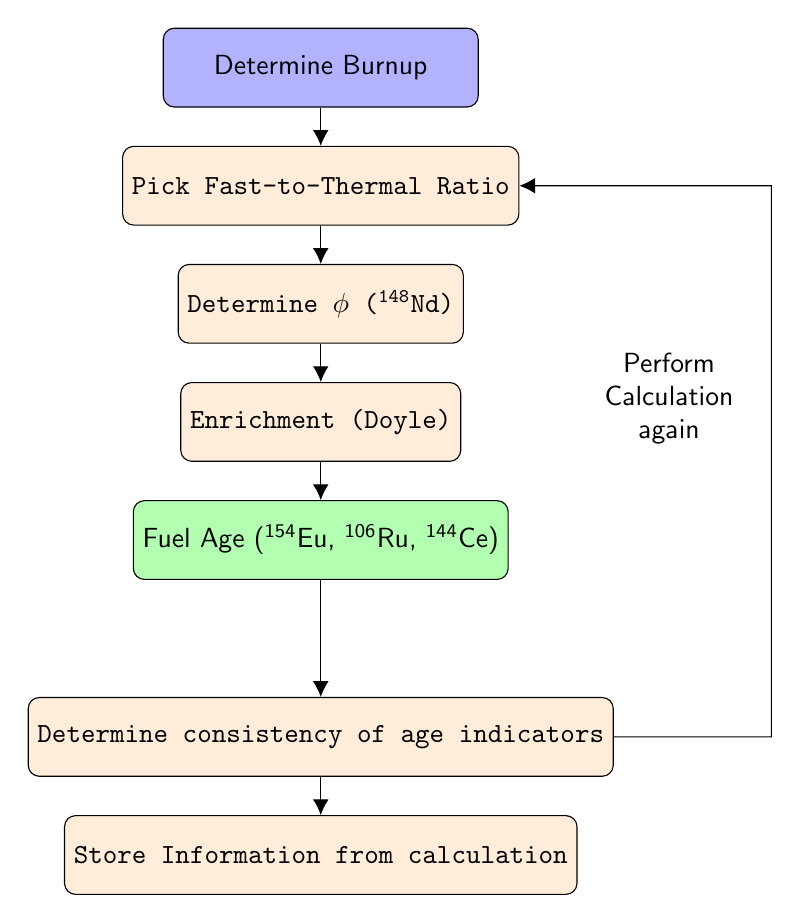
\begin{tikzpicture}[node distance=1.5cm,
    every node/.style={fill=white, font=\sffamily}, align=center]
  % Specification of nodes (position, etc.)
  \node (burnup)    [activityStarts]                {Determine Burnup};
  \node (Fast)      [process, below of=burnup]      {Pick Fast-to-Thermal Ratio};
  \node (phi)       [process, below of=Fast]        {Determine $\phi$ (\tss{148}Nd)};
  \node (rich)      [process, below of=phi]         {Enrichment (Doyle)};
  \node (age)       [activityRuns, below of=rich]   {Fuel Age (\tss{154}Eu, \tss{106}Ru, \tss{144}Ce)};
  \node (unity)     [process, below of=age, yshift=-1cm]
        {Determine consistency of age indicators};
  \node (store)     [process, below of=unity]       {Store Information from calculation};

  \draw[->]            (burnup) -- (Fast);
  \draw[->]              (Fast) -- (phi);
  \draw[->]               (phi) -- (rich);
  \draw[->]              (rich) -- (age);
  \draw[->]               (age) -- (unity);
  \draw[->]             (unity) -- (store);
  %% \draw[->]      (onPauseBlock) -- node {The activity is no longer visible}
  %%                                  (onStopBlock);
  %% \draw[->]       (onStopBlock) -- node {The activity is shut down by
  %%                                  user or system} (onDestroyBlock);
  %% \draw[->]    (onRestartBlock) -- (onStartBlock);
  %% \draw[->]       (onStopBlock) -| node[yshift=1.25cm, text width=3cm]
  %%                                  {The activity comes to the foreground}
  %%                                  (onRestartBlock);
  %\draw[->]    (onDestroyBlock) -- (ActivityDestroyed);
  %\draw[->]      (onPauseBlock) -| node(priorityXMemory)
  %                                 {higher priority $\rightarrow$ more memory}
  %                                 (ActivityEnds);
  %\draw           (onStopBlock) -| (priorityXMemory);
  %\draw[->]     (ActivityEnds)  |- node [yshift=-2cm, text width=3.1cm]
  %                                  {User navigates back to the activity}
  %                                  (onCreateBlock);
  \draw[->] (unity.east) -- ++(2,0) -- ++(0,5) -- ++(0,2) -- ++ (-3,0) --              
     node[xshift=1.8cm,yshift=-2.7cm, text width=2cm]
     {Perform Calculation again} (Fast.east);
  \end{tikzpicture}
\end{document}
